% default values
\def\ttau{0.01} % Zeitkonstante tau
%
% Plot Umgebung:
\def\samples{41}
%
\def\xomegaordermin{0}
\def\xomegaordermax{4}
\def\xomegamin{1e\xomegaordermin}
\def\xomegamax{1e\xomegaordermax}
\def\domain{\xomegamin:\xomegamax}
%
\def\yamptiefmin{0.8e-2}    % \ymin needed as macro to draw ycomb with node-text from x-axis to plot
\def\yamptiefmax{2}
%
\def\yamphochmin{0.8e-2}    % \ymin needed as macro to draw ycomb with node-text from x-axis to plot
\def\yamphochmax{2}
%
\def\yphitiefmax{+10}
\def\yphitiefmin{-100}      % \ymin needed as macro to draw ycomb with node-text from x-axis to plot % 1. Ordnung
\def\yphitiefg{-45}
%
\def\yphihochmin{-10}       % \ymin needed as macro to draw ycomb with node-text from x-axis to plot % 1. Ordnung % Alternative: [ycomb, update limits=false] small y value outer bounds but no dynamic node text
\def\yphihochmax{100}
\def\yphihochg{45}
%
%%%%%%%%%%%%%%%%%%%%%%%%%%%%%%%%%%%%%%%%%%%%%%%%%%%%%%%%%%%%%%%%%%%%%%%%%%%%
%
% RC-Tiefpass 1. Ord. Phasengang
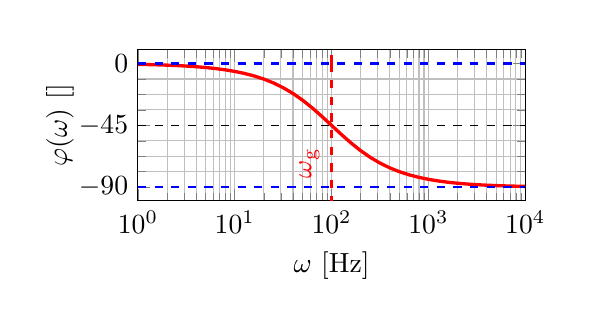
\begin{tikzpicture}[x=1mm,y=1mm] % gilt für tikz-coordinaten außerhalb der axis-environment

    \draw[draw=none] (-14,-12) rectangle (54,22); % Bildrahmen, Koordinatenbezug auf (0,0) des \begin{axis}...\end{axis} pgfplots, für

    \begin{semilogxaxis}[
        %title={Phasengang RC-Tiefpass 1. Ordnung},
        xlabel={$\omega\ [\mathrm{Hz}]$},
        ylabel={$\varphi(\omega)\ [\degree]$},
        ylabel shift = -5pt,
        xmin=\xomegamin, xmax=\xomegamax,
        ymin=\yphitiefmin, ymax=\yphitiefmax,
        ytick={0,-45,-90},
        domain=\domain,
        samples=\samples,
        minor y tick num= 3,
        log origin=infty,
        grid=minor,
        width=6.5cm,
        height=3.5cm,
    ]
        \addplot+[mark=none,very thick,red,]     {atan( -\x*\ttau) }; % Plot

        \addplot+[dashed,mark=none,black,]           coordinates { (\xomegamin, -45) (\xomegamax, -45) };%  node [pos=0.1,sloped,yshift=8pt] {$45\ \degree$};
        \addplot+[dashed,mark=none,blue,thick,]      coordinates { (\xomegamin, -90) (\xomegamax, -90) };%  node [pos=0.1,sloped,yshift=8pt] {$90\ \degree$};
        \addplot+[dashed,mark=none,blue,thick,]      coordinates { (\xomegamin, 0)  (\xomegamax, 0) };%   node [pos=0.1,sloped,yshift=8pt] {$0\ \degree$};
        \addplot+[ycomb,dashed,mark=none,thick,red,] coordinates { (1/(\ttau),\yphitiefmin) (1/(\ttau),\yphitiefmax) } node [pos=0.25,sloped,style={yshift=8pt}] {$\omega_{\mathrm{g}}$};

    \end{semilogxaxis}%
\end{tikzpicture}%